\documentclass[12pt]{article}
\usepackage[utf8]{inputenc}
\usepackage{amsmath}
\usepackage{amsfonts}
\usepackage{amsthm}
\usepackage{amssymb}
\usepackage{alltt}
\usepackage{array}
\usepackage[backend=bibtex,style=ieee,]{biblatex}
\usepackage{blindtext}
\usepackage{bold-extra}
\usepackage{caption}
\usepackage{copyrightbox}
\usepackage{dirtree}
\usepackage{enumitem}
\usepackage{float}
\usepackage{geometry}
\usepackage{graphicx}
\usepackage{hyperref}
\usepackage{indentfirst}
\usepackage[newfloat]{minted}
\usepackage{multicol}
\usepackage{multirow}
\usepackage{latexsym}
\usepackage{listings}
\usepackage{pdfpages}
\usepackage{setspace}
\usepackage{url}
\usepackage{wrapfig}
\usepackage{titlesec}
\usepackage[most]{tcolorbox}
\usepackage{xifthen}
\usepackage{xparse}

% First the counter, Second the number
\newcommand{\addnumbertofigure}[1]{\addtocounter{figure}{#1}\thefigure \addtocounter{figure}{-#1}}

\geometry{
  a4paper
}

% Setting section depth for some use case
% \setcounter{tocdepth}{5}
% \setcounter{secnumdepth}{4}

% Title related settings
\newcommand{\titleItem}[2]{
  \large{
    \textbf{#1}
  } \\
  \large{
    #2
  } \\
  \vspace{8pt}
}

% \titleformat{\paragraph}
% {\normalfont\normalsize\bfseries}{\theparagraph}{1em}{}
% \titlespacing*{\paragraph}
% {0pt}{3.25ex plus 1ex minus .2ex}{1.5ex plus .2ex}

% Updating array stretch for tables
\renewcommand{\arraystretch}{2}

% Increasing the spacing
\doublespacing

% References
\bibliography{references}

\begin{document}

\begin{titlepage}
  \begin{center}

  % Main title
  \begin{figure}[ht]
    \begin{minipage}[l]{.09\textwidth}
      
\includegraphics[width=\linewidth]{img/metu-logo.png}
    \end{minipage}
    \begin{minipage}[c]{.8\textwidth}
      \centering
      \large{
        \textbf{MIDDLE EAST TECHNICAL UNIVERSITY}
      }

      \normalsize{
        \textbf{DEPARTMENT OF COMPUTER ENGINEERING}
      }
    \end{minipage}
    \begin{minipage}[r]{.09\textwidth}
      
\includegraphics[width=\linewidth]{img/metu-ceng-logo.png}
    \end{minipage}
  \end{figure}
  
  % Logo of project
  \begin{figure}[ht]
    \centering
    
\includegraphics[width=.5\linewidth]{img/afetbilgi.jpg}
  \end{figure}

  % Name of report
  \vspace{16pt}
  \large{
    \textbf{SOFTWARE ARCHITECTURE DESCRIPTION (SAD)}
  } \\
  \large{
    \textbf{SPRING 2022-2023}
  }

  % Nape of the project
  \rule{12cm}{1pt}
  % \vspace{-7pt}

  \large{\textbf{afetbilgi.com}}
  \vspace{-7pt}

  \rule{12cm}{1pt}
  
  % Group Name
  \vspace{24pt}
  \Large{\textbf{Group 24}}

  % Names of the students
  \vspace{48pt}
  \begin{minipage}{.45\textwidth}
    \centering
    \titleItem{Burak Metehan Tunçel}{2468726}
  \end{minipage}
  \hfill
  \begin{minipage}{.45\textwidth}
    \centering
    \titleItem{Saad Yousuf}{2349819}
  \end{minipage}  
  \end{center}
\end{titlepage}
  

\newpage

\tableofcontents

\newpage

\listoffigures

\newpage

\listoftables

\newpage

\section{Introduction}

\subsection{Purpose of the System}

\subsection{Scope}

\subsection{System Overview}

\subsubsection{System Perspective}

\begin{figure}[H]
  \centering
  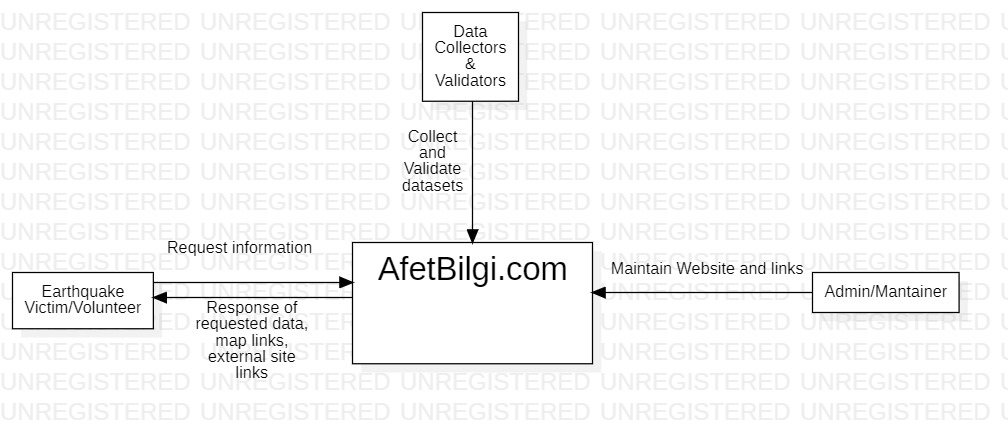
\includegraphics[width=\textwidth]{img/context-diagram.jpg}
  \caption{Context Diagram for \href{https://afetbilgi.com}{afetbilg.com}}
\end{figure}

\subsubsection{System Functions}

\subsubsection{Stakeholder Characteristics}

\subsubsection{Limitations}

\subsection{Definitions}


\newpage

\section{References}


\newpage

\section{Specific Requirements}

\subsection{External Interfaces}

\begin{figure}[H]
    \centering
    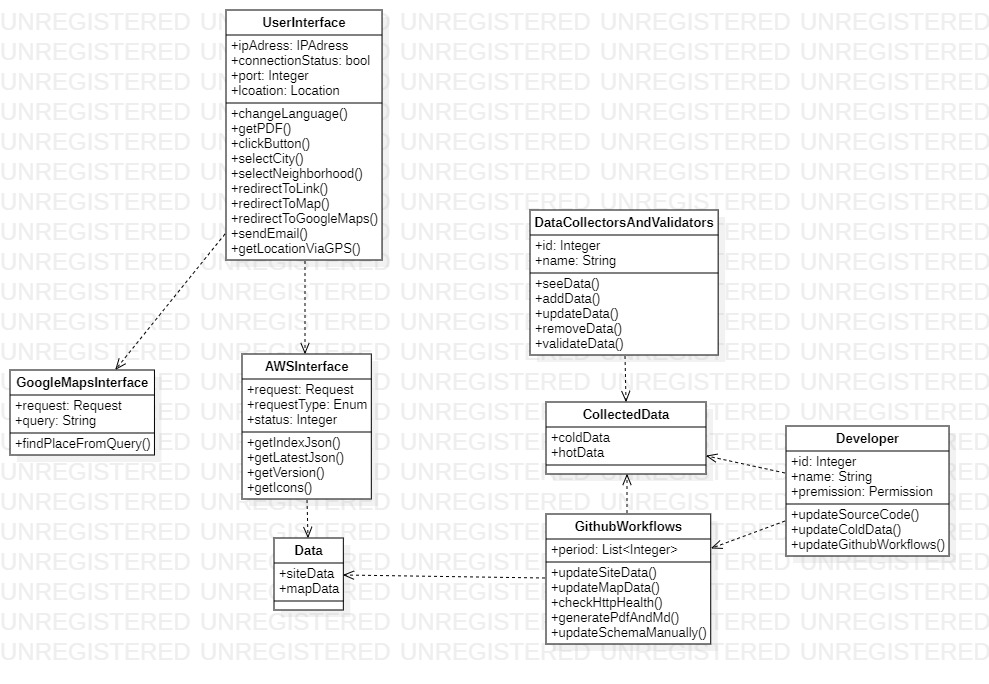
\includegraphics[width=\textwidth]{img/external-interfaces.jpg}
    \caption{External Interfaces}
\end{figure}

\subsection{Functions}

\begin{figure}[H]
  \centering
  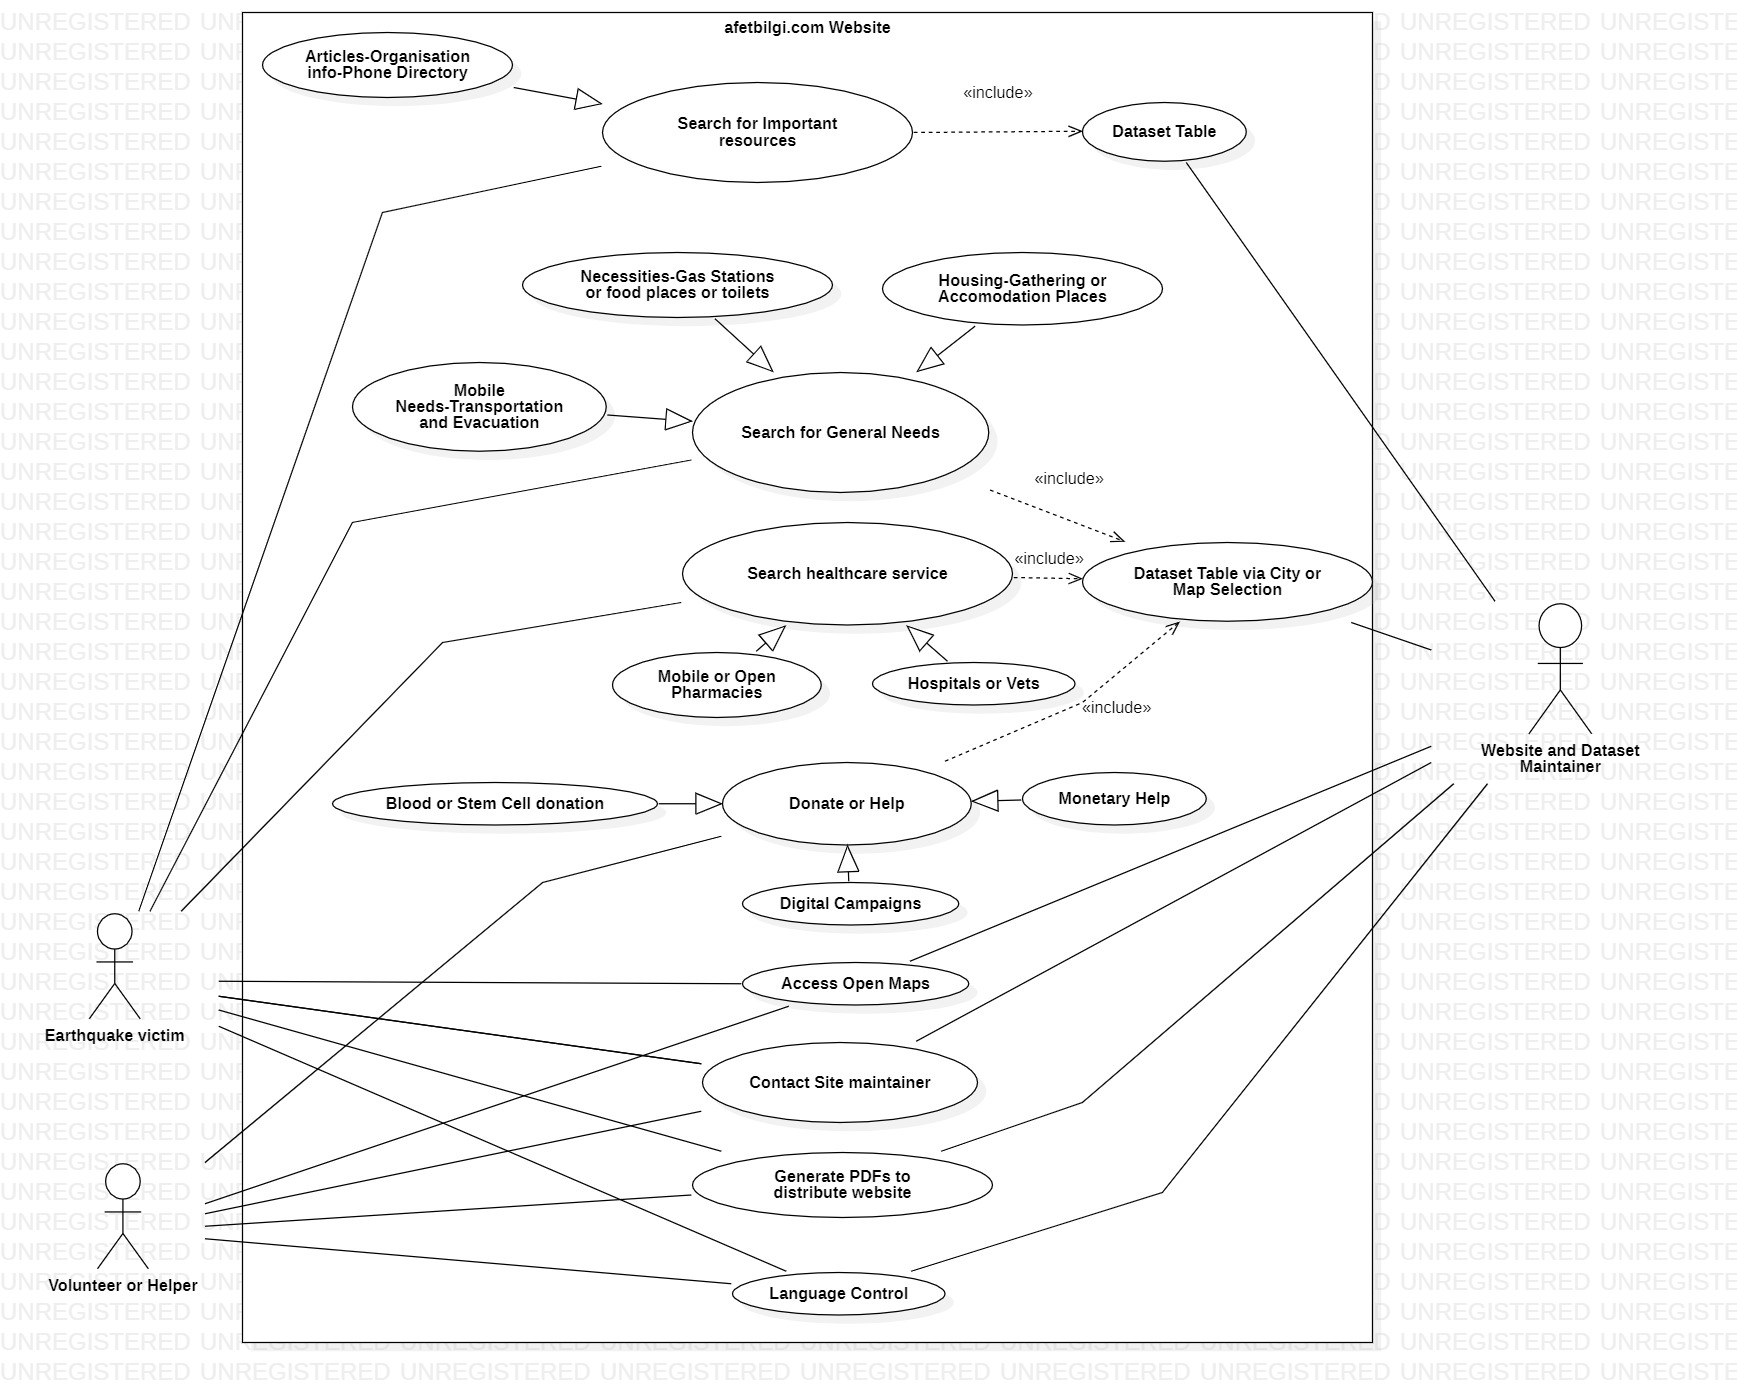
\includegraphics[width=\textwidth]{img/use-case-diagram.jpg}
  \caption{Use Case Diagram for \afetbilgi}
\end{figure}

\begin{table}[H]
  \centering
  \begin{tabular}{|p{.3\linewidth}|p{.7\linewidth}|}
    \hline
    \textbf{Use Case ID} & \thetable \\
    \hline
    \textbf{Use-Case Name} & Donate or Help \\
    \hline
    \textbf{Actors} & Volunteer or Helper and Website maintainers \\
    \hline
    \textbf{Description} & Whenever a site user wants to donate or help earthquake victims, he or she can view verified and updated institutions and organisations, which he or she can donate to, on the website to donate to \\
    \hline
    \textbf{Data} & Verified and updated directory of external 3rd party links of welfare and governmental organisations \\
    \hline
    \textbf{Preconditions} & The directory must be updated and verified regularly given the potential monetary usage of the links in the future by the users \\
    \hline
    \textbf{Stimulus} & User clicks on the relevant donation/help methods listed as bold text buttons in the ``\texttt{To Help}'' category on the website \\
    \hline
    \textbf{Basic Flow} & 
        \begin{minipage}[ht]{\linewidth} 
            \begin{enumerate}[label=\textbf{Step \arabic*:},leftmargin=1.5\leftmargin]
                \item User clicks on ``\texttt{Digital solidarity campaigns}''
                \item User selects any of the presented external-3rd party links(presented in a directory)
                \item User redirected to verified 3rd party website
            \end{enumerate}
        \end{minipage} \\
    \hline
    \textbf{Alternative Flow \#1} & 
        \begin{minipage}[ht]{\linewidth} 
            \begin{enumerate}[label=\textbf{Step \arabic*:},leftmargin=1.5\leftmargin]
                \item User clicks on ``\texttt{Other donation}''
                \item User selects relevant city
                \item User selects verified helper links of individuals/smaller organisations along with their contact details
                \item User clicks on any link and escorted out to a 3rd party site
            \end{enumerate}
        \end{minipage} \\
    \hline
    \textbf{Alternative Flow \#2} &
    \begin{minipage}[ht]{\linewidth} 
            \begin{enumerate}[label=\textbf{Step \arabic*:},leftmargin=1.5\leftmargin]
                \item User clicks on ``\texttt{Kizilay Blood Donation Places}''
                \item User automatically redirected to primary verified 3rd party site of governmental organisation accepting blood donations
            \end{enumerate}
        \end{minipage} \\
    \hline
    \textbf{Exception Flow} & - \\
    \hline
    \textbf{Post Conditions} & User is redirected to a verified external website out of the afetbilgi.com domain \\
    \hline
  \end{tabular}
  \caption{Use Case - Donate or Help}
\end{table}

\begin{table}[H]
  \centering
  \begin{tabular}{|p{.3\linewidth}|p{.7\linewidth}|}
    \hline
    \textbf{Use Case ID} & \thetable \\
    \hline
    \textbf{Use-Case Name} & Access open maps \\
    \hline
    \textbf{Actors} & Volunteers or Victims, Website maintainers \\
    \hline
    \textbf{Description} & Users can view current location with respect to places in need of help and use interactive map view to track down relevant places offering help (verified by site maintainers) via GPS location \\
    \hline
    \textbf{Data} & Interactive Map View with relevant place descriptions to navigate on \\
    \hline
    \textbf{Preconditions} & Places ought to be verified, properly categorised and color coded for easy understanding by site user \\
    \hline
    \textbf{Stimulus} & User drags mouse around on map view involving GPS after clicking on the map button anywhere on screen or calling \href{https://maps.afetbilgi.com}{\texttt{maps.afetbilgi.com}} directly in the browser \\
    \hline
    \textbf{Basic Flow} & 
        \begin{minipage}[ht]{\linewidth} 
            \begin{enumerate}[label=\textbf{Step \arabic*:},leftmargin=1.5\leftmargin]
                \item User is shown his current location with respect to to rest of Turkey
                \item Users can zoom in or out of Turkey's map and track themselves to needy areas as per color codes and categorisation
                \item User can click on a tracked down helping house, restaurant, etc. and be greeted by a pop up box with description and relevant links to third party sites or Google Maps routes
                \item User can click on the links and escorted out to 3rd party websites or Google Maps website
            \end{enumerate}
        \end{minipage} \\
    \hline
    \textbf{Alternative Flow \#1} & 
    \begin{minipage}[ht]{\linewidth} 
            \begin{enumerate}[label=\textbf{Step \arabic*:},leftmargin=1.5\leftmargin]
                \item User can select zoom in or out along with clicking on the camera icon
                \item User can save map screenshot for later use or distribution
            \end{enumerate}
        \end{minipage} \\
    \hline
    \textbf{Alternative Flow \#2} & - \\
    \hline
    \textbf{Exception Flow} & - \\
    \hline
    \textbf{Post Conditions} & User ends up on verified external website outside of \afetbilgi domain \\
    \hline
  \end{tabular}
  \caption{Use Case - Access open maps}
\end{table}

\begin{table}[H]
  \centering
  \begin{tabular}{|p{.3\linewidth}|p{.7\linewidth}|}
    \hline
    \textbf{Use Case ID} & \thetable \\
    \hline
    \textbf{Use-Case Name} & Generate PDFs to distribute website \\
    \hline
    \textbf{Actors} & Volunteers or victims \\
    \hline
    \textbf{Description} & Users can save filtered out website directories for later use given possible lack of electrical or network necessities in these earthquake stricken areas\\
    \hline
    \textbf{Data} & Separate downloadable PDF documents after selecting relevant cities \\
    \hline
    \textbf{Preconditions} & User is able to select entire cities with verified directory links and contact information  \\
    \hline
    \textbf{Stimulus} & User clicks on PDF icon button anywhere on the website \\
    \hline
    \textbf{Basic Flow} &
        \begin{minipage}[ht]{\linewidth} 
            \begin{enumerate}[label=\textbf{Step \arabic*:},leftmargin=1.5\leftmargin]
                \item User clicks on PDF icon anywhere on website
                \item User selects city
                \item Document is loaded and enabled for download by the user with the relevant city and categories highlighted on it
            \end{enumerate}
        \end{minipage} \\
    \hline
    \textbf{Alternative Flow \#1} & - \\
    \hline
    \textbf{Alternative Flow \#2} & - \\
    \hline
    \textbf{Exception Flow} & - \\
    \hline
    \textbf{Post Conditions} & Site user has received well formatted and legible generated PDF document with relevant hyperlinks and contact details of verified directories  \\
    \hline
  \end{tabular}
  \caption{Use Case - Generate PDFs to distribute website}
\end{table}

\subsection{Usability Requirements}

\subsection{Performance Requirements}

\subsection{Logical Database Requirements}

\afetbilgi does not currently have any relational database. To acquire the required data for both site and maps, it gets a JSON file from AWS and the code of website parses this JSON file according the path and the chosen option. For this purpose, it uses axios to send \texttt{GET} request to the \href{https://cdn.afetbilgi.com/latest.json}{\texttt{cdn.afetbilgi.com/latest.json}}. This request returns the \texttt{latest.json} file, which includes all the data required in the website. Although it may have drawback such as long load time, it may have advantages such as not loading any data after initial load.

To parse and upload the JSON file into the AWS, Github Workflows are used. Github Workflows parse and upload the \texttt{latest.json} by using the data, which collectors and validators collect and validate, periodically.

The relations between objects in the JSON file is shown at Figure \addnumbertofigure{1}. The code use these relations to parse the JSON correctly and show the included information in the JSON. If the system is updated to a relational database, the database can use the relations at the Figure \addnumbertofigure{1}.

\begin{figure}[H]
    \centering
    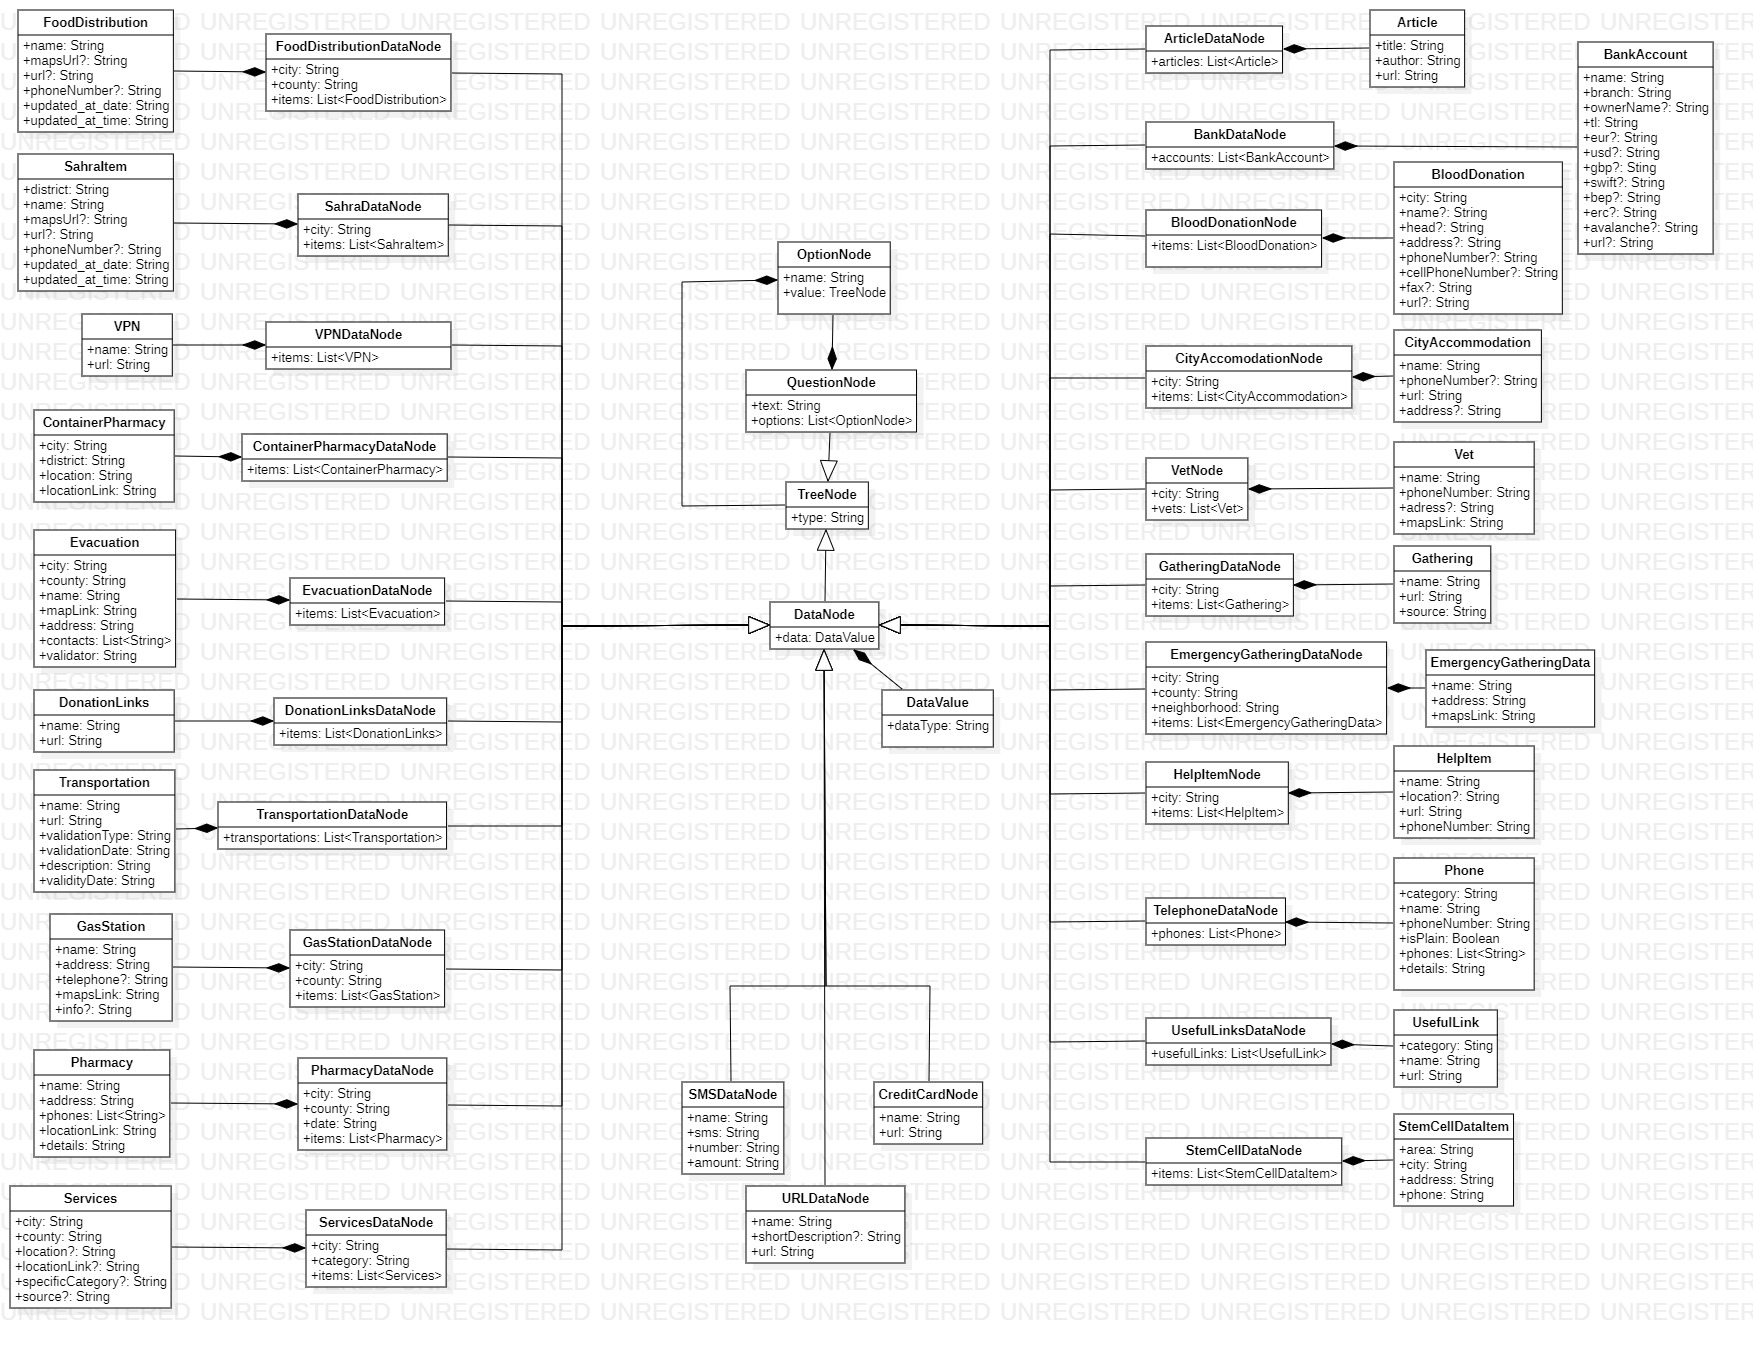
\includegraphics[width=\textwidth]{img/database.jpg}
    \caption{Possible Relational Database}
\end{figure}

\subsection{Design Constraints}

\subsection{System Attributes}

\subsection{Supporting Information}


\newpage

\section{Suggestions to Improve the Existing System}

\subsection{System Perspective}

% Checked in grammarly
\afetbilgi is not part of a more extensive system. It is a standalone and open-source efforted website to verify critical information in the fight against the 6 February 2023 Pazarcik Earthquake and deliver it to disaster victims and those who want to help in an understandable, concise manner in multiple languages.

This information is presented in either the form of legible tables with third-party governmental and private links or an interactable method via a map view interface. If deemed necessary, admin and maintainers can make changes to display newly created or edited data and upload it to the system upon any complaints or suggestions they may get on their contact details.

\begin{figure}[H]
  \centering
  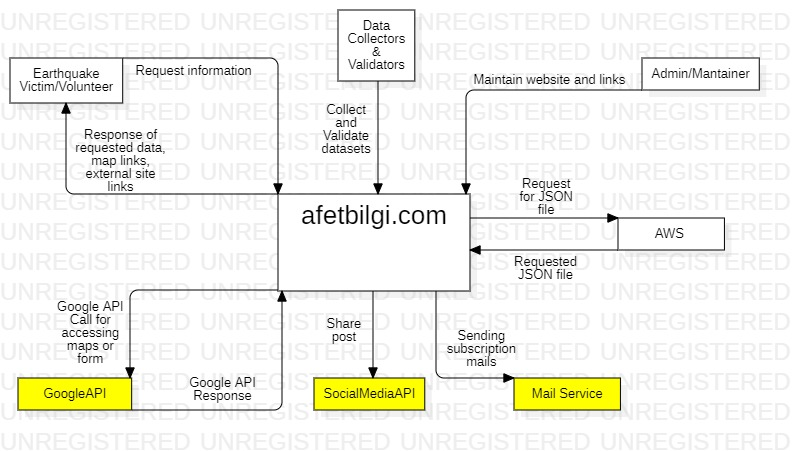
\includegraphics[width=\linewidth]{img/context-diagram-s4.jpg}
  \caption{Context Diagram for \afetbilgi}
\end{figure}

\vfill
\newpage

The \afetbilgi\ consists of a combination of small physical and software parts. With the help of interfaces, these parts communicate among themselves and with the user. The following are the interfaces through which interaction occurs:
\begin{itemize}
  \setlength{\itemsep}{1pt}
  \item User interfaces
  \item Software interfaces
  \item Communication interfaces
\end{itemize}
Users interact with the website through their devices connected to the internet, such as cell phones or computers, as the user interface. The software interface enables the website to serve additional features to the user.

\subsubsection{User Interfaces}

In order to start using the website, a user should go into the website via a device connected to the internet. The website may have some loading time. After loading, the website is ready for user interactions. Users can interact with \afetbilgi\ directly to access required information.

The user interface contains \href{https://mui.com/}{MUI} components which are clear buttons and lists. Users can interact with the buttons to access the list of information or access more options related to the chosen information type.

\subsubsection{Software Interfaces}

\afetbilgi\ runs mainly JavaScript code with React library. It also uses additional react libraries such as \href{https://mui.com/}{MUI}.

The website makes necessary request to use some features such as accessing Google API, social media APIs and mail service.

\subsubsection{Communication Interfaces}

Since \afetbilgi\ is a website, it communicates via HTTPS (Hypertext Transfer Protocol Secure) and underlying protocols such as TCP/IP. It uses HTTPS to access APIs and servers.

\subsection{External Interfaces}

\vfill
\begin{figure}[H]
  \centering
  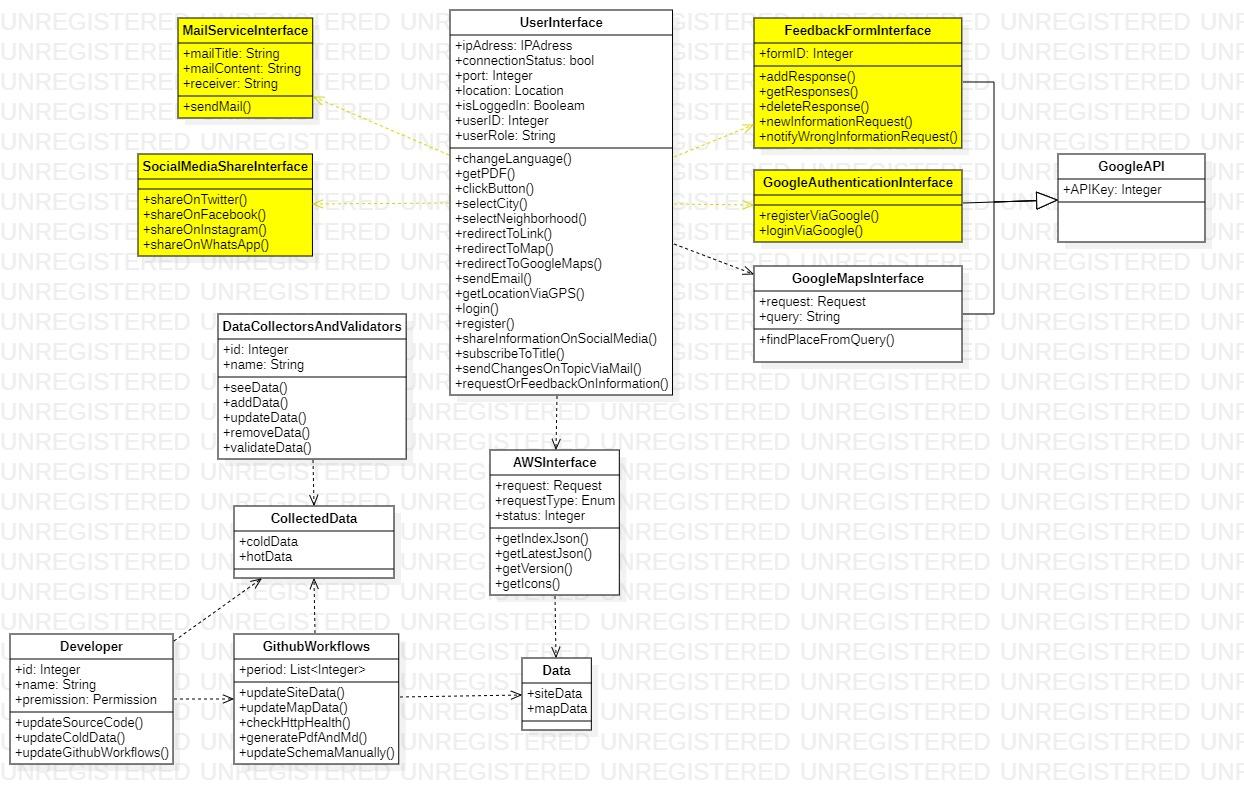
\includegraphics[width=\linewidth]{img/external-interfaces-s4.jpg}
  \caption{Suggested New External Interfaces}
\end{figure}
\vfill
\newpage

\subsection{Functions}

\subsection{Usability Requirements}

\subsection{Performance Requirements}

\subsection{Logical Database Requirements}

\afetbilgi\ does currently have a relational database. To make minor difference in the source code, the object structure in the Section 3.5 is preserved. Additionally, users, roles and mail subscription data are added into database. \texttt{Users} relation provides information related to the login system. \texttt{Roles} relation provides information related to the registered role. \texttt{Mail Subscription} relation provides the information related to topics that users subcribed. \texttt{SiteInformation} relation provides information related to the information located in the website.

\begin{figure}[H]
  \centering
  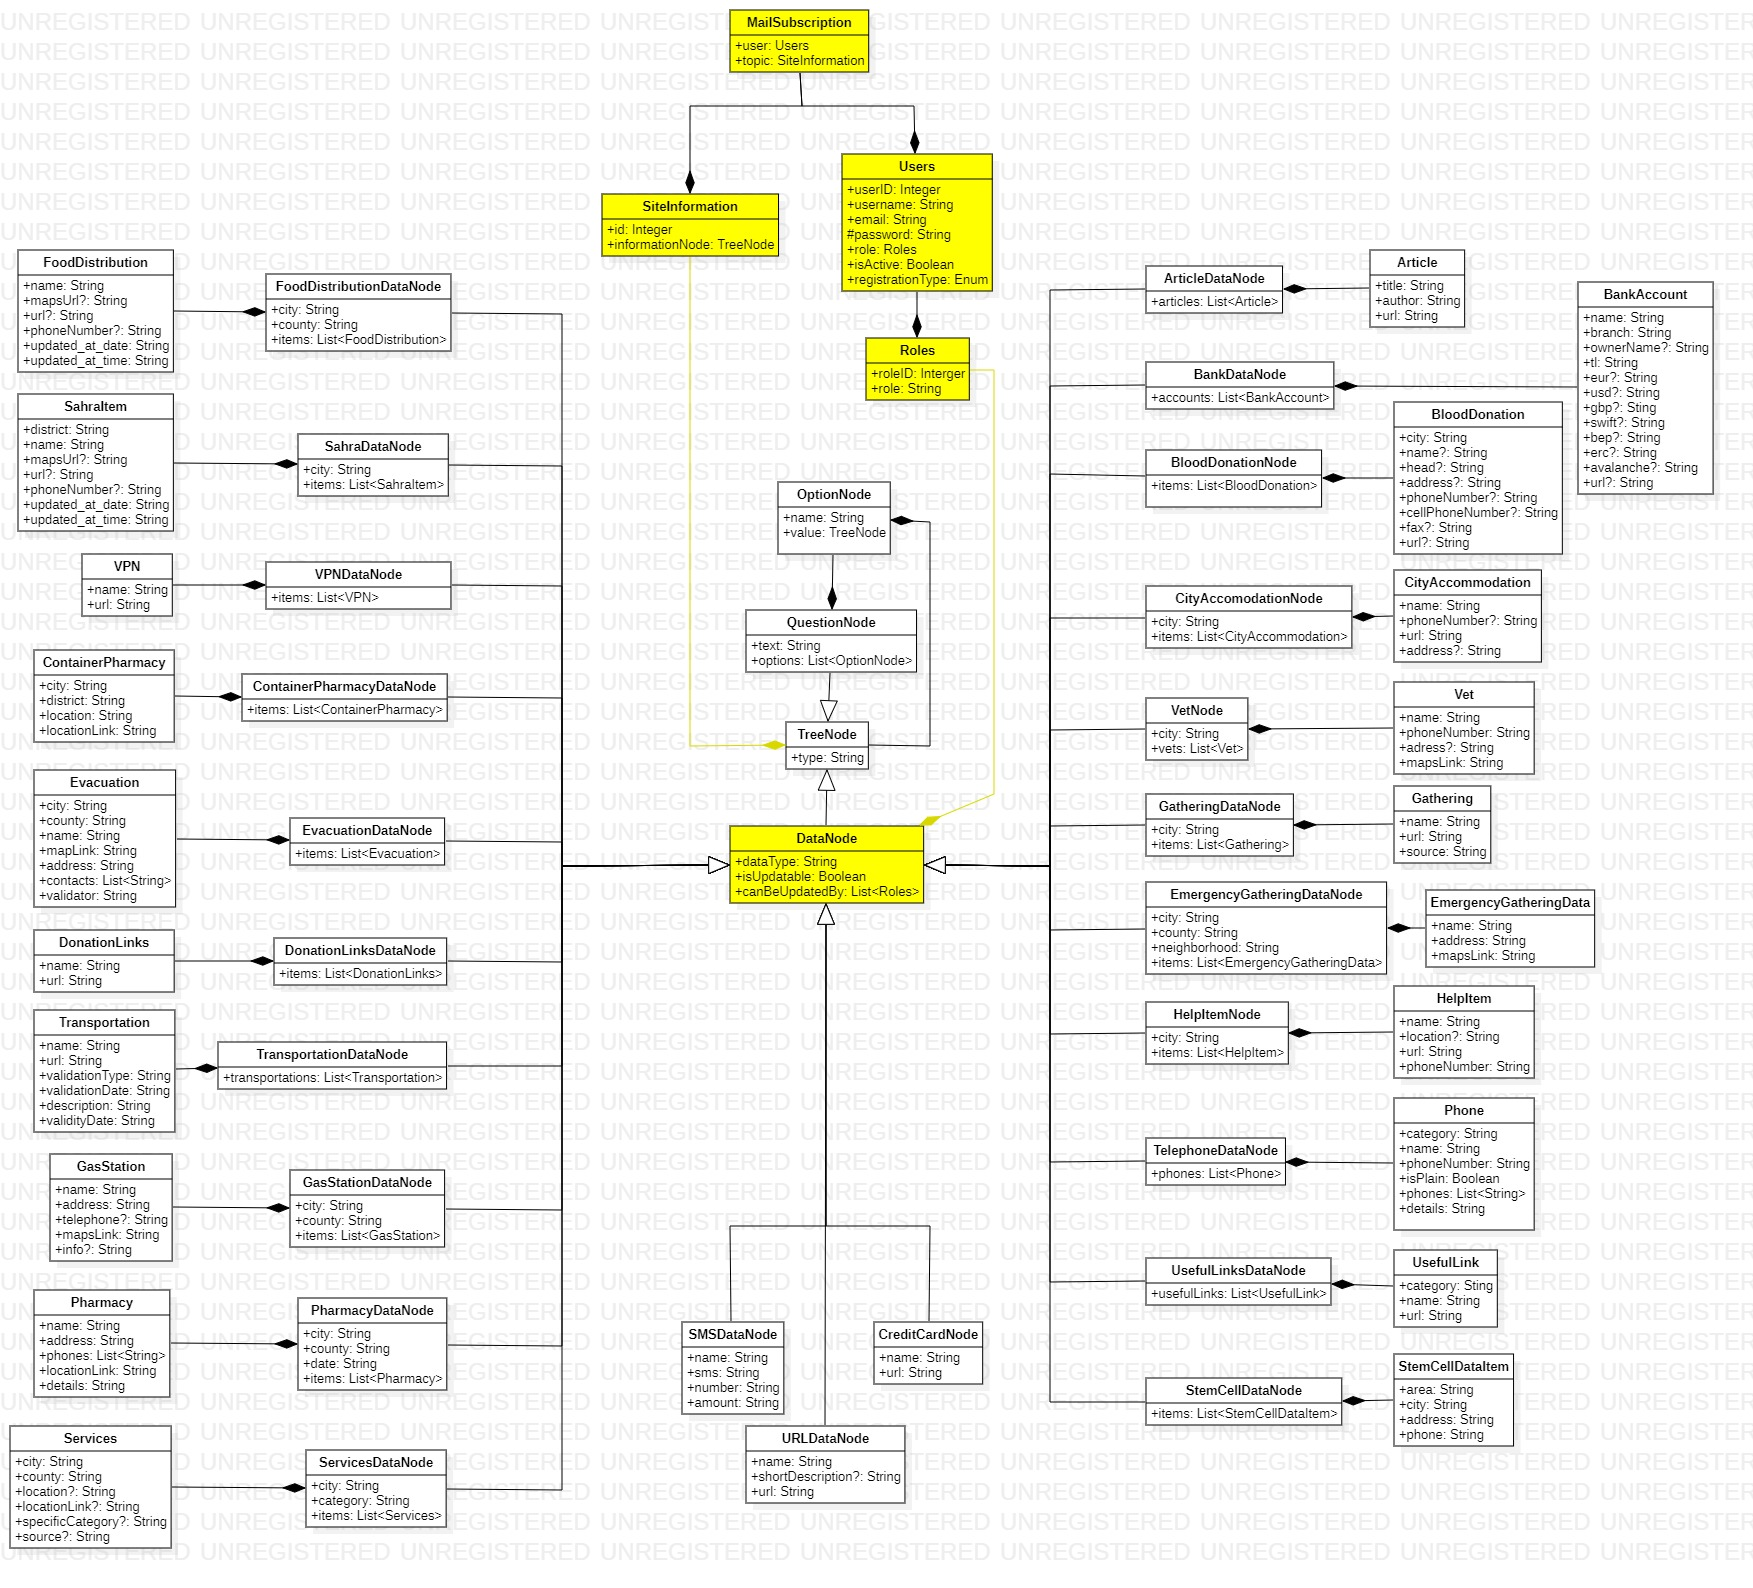
\includegraphics[width=\linewidth]{img/database-s4.jpg}
  \caption{Suggested New Relational Database}
\end{figure}

\subsection{Design Constraints}

\subsection{System Attributes}

\subsection{Supporting Information}


\end{document}
